\section{Empirical Results and Comparative Analysis}
\label{section:results}

\subsection{Master Benchmark Results}
Table~\ref{tab:benchmark_master} compiles the primary empirical results across all architectures evaluated on CIFAR-100 alongside the Week 02 baselines.

\begin{table}[htbp]
\centering
\begin{adjustbox}{max width=\textwidth}
\small
\setlength{\tabcolsep}{5pt}
\begin{tabular}{lllrcrr}
\toprule
\textbf{Model Architecture} & \textbf{Paradigm} & \textbf{Spatial Token Mixer} & \textbf{Params} & \textbf{Epochs} & \textbf{Top-1 Val (\%)} & \textbf{Train Time} \\
\midrule
ResMLP Baseline & Isotropic & Pure Linear $(N \times N)$ & 2.19M & 100 & 62.40\% & 54.6 min \\
RepMLP Baseline & Hierarchical & RepConv 3-Branch & 2.16M & 100 & 71.46\% & 107.1 min \\
\textbf{Pyramid-ResMLP Pure} & Hierarchical & Linear $(N_i \times N_i)$ & \textbf{1.93M} & 100 & \textbf{68.22\%} & \textbf{44.9 min} \\
\textbf{Pyramid-ResMLP} & Hierarchical & RepToken (Fused)$^*$ & \textbf{1.79M} & 100 & \textbf{72.18\%} & \textbf{44.5 min} \\
\textbf{Shift-ResMLP} & Isotropic & 4-Direction Shift & 14.26M & 100 & \textbf{72.92\%} & 110.2 min \\
\textbf{CA-Mixer} & Isotropic NCA & Cellular Automata & \textbf{1.90M} & 100 & \textbf{64.92\%} & \textbf{58.4 min} \\
PoolFormer-S12 & Hierarchical & Non-parametric AvgPool$^\dagger$ & 11.45M & 100 & 59.50\% & $\sim$53 min \\
HybridFormer & Hierarchical & PoolFormer + MHSA & 10.59M & 300 & \textbf{75.70\%} & $\sim$160 min \\
\bottomrule
\end{tabular}
\end{adjustbox}
\vspace{0.4em}
\caption{Empirical performance benchmark on CIFAR-100 across architectural paradigms. $^*$Pyramid-ResMLP contains 1.94M training parameters (1,938,820) which structurally fuse into 1.79M (1,785,828) upon deployment. CA-Mixer scales to 64.92\% Top-1 validation accuracy at 1.90M parameters (1,901,100 params, 0.489 GFLOPs, 2.20\% ECE, 58.4 min) over 100 epochs, compared to 62.87\% in the 30-epoch 1.21M fast exploration (20.0 min). $^\dagger$PoolFormer-S12 is evaluated at $224 \times 224$ following the canonical MetaFormer training setup~\cite{yu2022metaformer}.}
\label{tab:benchmark_master}
\end{table}

\subsection{Training Dynamics and Learning Profiles}
Because experimental schedules varied across paradigms (100 epochs for our primary models, 30 epochs for rapid CA-Mixer exploration, and 300 epochs for HybridFormer), we analyze their learning trajectories based on their respective optimization dynamics and generalization behavior.

\begin{figure}[htbp]
\centering
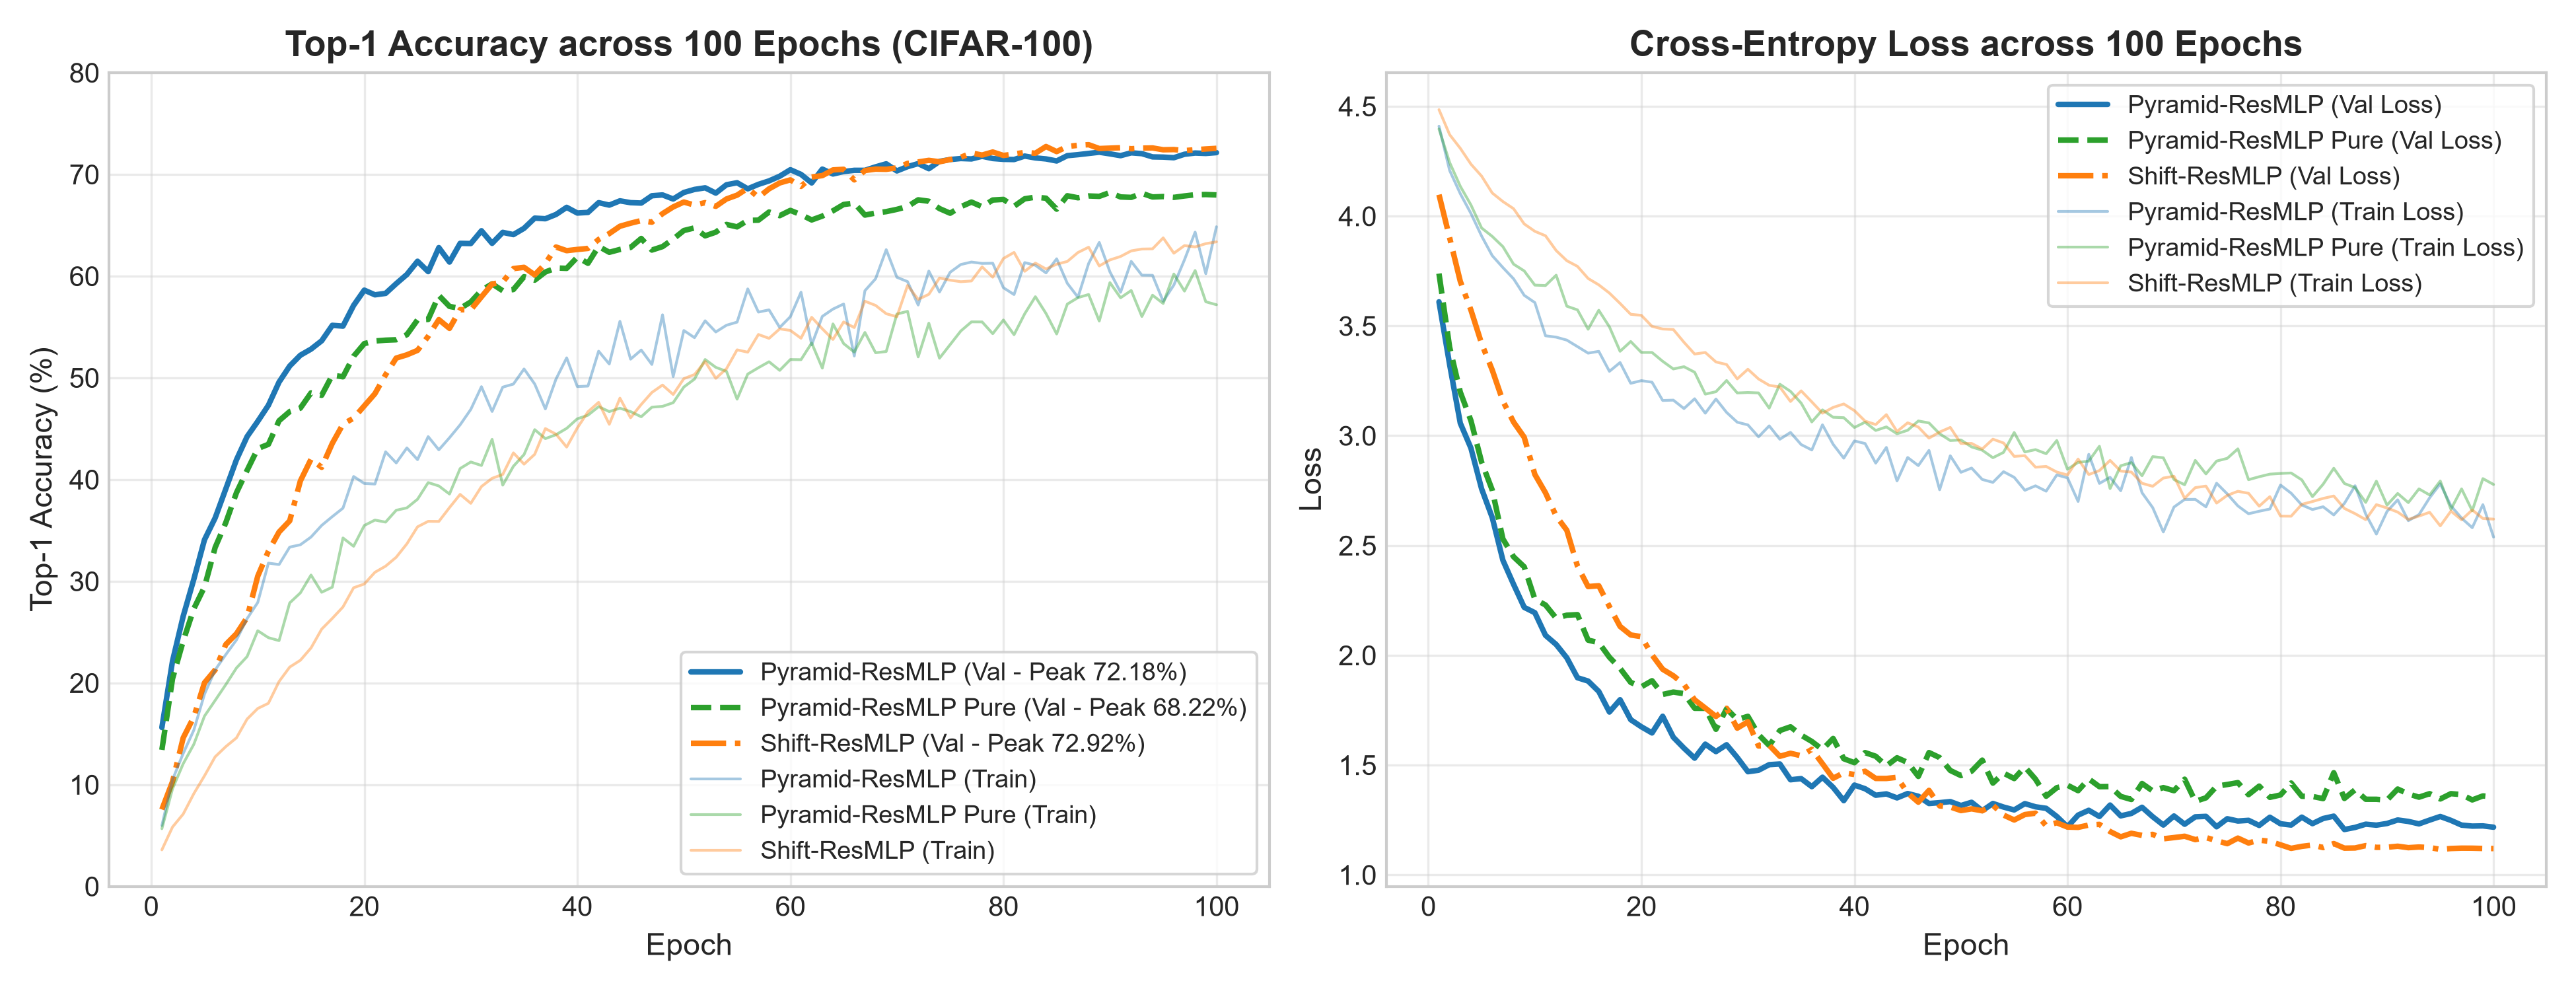
\includegraphics[width=\textwidth]{figures/training_curves_comparison.png}
\caption{Training and validation dynamics across 100 epochs on CIFAR-100 comparing Pyramid-ResMLP, Pyramid-ResMLP Pure, and Shift-ResMLP.}
\label{fig:curves_comparison}
\end{figure}

\subsubsection{Convergence Behavior of Pyramid Models and Shift-ResMLP}
Figure~\ref{fig:curves_comparison} compares the Top-1 validation accuracy and cross-entropy loss trajectories for our three 100-epoch CIFAR-100 runs. Table~\ref{tab:epoch_progress} provides numerical checkpoints partitioned into validation accuracy and cross-entropy loss trajectories.

\begin{table}[htbp]
\centering
\begin{subtable}{\textwidth}
\centering
\small
\begin{tabularx}{\textwidth}{c*{3}{>{\centering\arraybackslash}X}}
\toprule
\textbf{Epoch} & \textbf{Pyramid-ResMLP Pure} & \textbf{Pyramid-ResMLP} & \textbf{Shift-ResMLP} \\
\midrule
1  & 13.42\% & 15.62\% & 7.56\% \\
10 & 43.04\% & 45.72\% & 30.50\% \\
20 & 53.36\% & 58.62\% & 47.24\% \\
40 & 61.86\% & 66.20\% & 62.62\% \\
60 & 66.46\% & 70.46\% & 69.46\% \\
80 & 67.54\% & 71.48\% & 71.86\% \\
\midrule
\textbf{Peak} & \textbf{68.22\%} (Epoch 90) & \textbf{72.18\%} (Epoch 89) & \textbf{72.92\%} (Epoch 88) \\
100 & 67.98\% & 72.14\% & 72.56\% \\
\bottomrule
\end{tabularx}
\vspace{0.3em}
\caption{Top-1 Validation Accuracy Trajectory (\%).}
\label{tab:val_acc_trajectory}
\end{subtable}

\vspace{0.8em}

\begin{subtable}{\textwidth}
\centering
\small
\begin{tabularx}{\textwidth}{c*{3}{>{\centering\arraybackslash}X}}
\toprule
\textbf{Epoch} & \textbf{Pyramid-ResMLP Pure} & \textbf{Pyramid-ResMLP} & \textbf{Shift-ResMLP} \\
\midrule
1  & 3.7385 & 3.6098 & 4.0979 \\
10 & 2.2554 & 2.1938 & 2.8236 \\
20 & 1.8562 & 1.6741 & 2.0848 \\
40 & 1.5107 & 1.4088 & 1.4567 \\
60 & 1.4081 & 1.2189 & 1.2175 \\
80 & 1.3638 & 1.2324 & 1.1366 \\
\midrule
\textbf{Peak} & \textbf{1.3402} (Epoch 90) & \textbf{1.2262} (Epoch 89) & \textbf{1.1330} (Epoch 88) \\
100 & 1.3546 & 1.2169 & 1.1197 \\
\bottomrule
\end{tabularx}
\vspace{0.3em}
\caption{Validation Cross-Entropy Loss Trajectory.}
\label{tab:val_loss_trajectory}
\end{subtable}
\vspace{0.5em}
\caption{Validation convergence dynamics across 100 epochs on CIFAR-100, comparing (a) Top-1 validation accuracy (\%) and (b) validation cross-entropy loss trajectories between Pyramid-ResMLP Pure, Pyramid-ResMLP, and Shift-ResMLP.}
\label{tab:epoch_progress}
\end{table}

Key observations from the training curves include:
\begin{itemize}
    \item \textbf{Regularization inverted gap in early epochs:} In all three models, training accuracy appears lower than validation accuracy for the first 40 epochs. This is expected behavior caused by heavy data augmentations (Mixup with $\alpha=0.8$, CutMix with $\alpha=1.0$, and RandAugment), which corrupt training images to prevent early memorization, while validation evaluation runs on clean images.
    \item \textbf{Accelerated convergence of Pyramid-ResMLP:} Pyramid-ResMLP consistently outpaces Pyramid-ResMLP Pure by $3-5\%$ throughout the training run. By epoch 20, Pyramid-ResMLP achieves 58.62\% validation accuracy, whereas Pyramid-ResMLP Pure reaches 53.36\% and Shift-ResMLP reaches 47.24\%.
    \item \textbf{Late-epoch stabilization:} All three models reach their peak performance between epochs 88 and 90, corresponding to the final annealing phase of the Cosine learning rate schedule where the step size reaches $\eta_{\text{min}} = 10^{-6}$.
\end{itemize}

\subsubsection{Convergence Dynamics and 100-Epoch Scaling in CA-Mixer}
To rigorously evaluate whether Neural Cellular Automata token mixing scales with model capacity and extended training schedules, CA-Mixer was benchmarked under two distinct regimes:
\begin{itemize}
    \item \textbf{Compact 30-epoch rapid exploration (1.21M parameters):} Processing in-memory GPU tensors without data augmentation bottlenecks required only 20.0 minutes across three random seeds ($62.87 \pm 0.24\%$ Top-1 validation accuracy, $88.09 \pm 0.30\%$ Top-5). CA-Mixer constrained the train-test generalization gap to $20.74 \pm 0.56\%$ (slashing overfitting by over 17\% compared to unconstrained dense mixers) and attained an Expected Calibration Error (ECE) of $3.82 \pm 0.22\%$.
    \item \textbf{Parameter-matched 100-epoch scaling (1.90M parameters):} Scaling CA-Mixer to 1.90M parameters ($C=160, D=6, C_{\text{nca}}=160, C_{\text{channel}}=652$) directly matches the parameter budget of Pyramid-ResMLP Pure (1.93M) and Pyramid-ResMLP (1.94M train / 1.79M deploy). When trained for 100 epochs with AdamW ($\eta = 10^{-3}, \lambda = 0.05$) and dynamic step jitter ($T_{\text{jitter}}=0.25$, $T=4$ at $32\times32$, 0.489 GFLOPs/image), CA-Mixer achieves \textbf{64.92\%} Top-1 accuracy, \textbf{85.72\%} Top-5 accuracy, and a test loss of $1.503$ in 58.4 minutes (35.0 seconds/epoch, 3,942 images/second on a single Tesla T4 GPU, Figure~\ref{fig:ca_100ep_curves}). Furthermore, the Expected Calibration Error is reduced to an outstanding \textbf{2.20\%}, establishing CA-Mixer as the most well-calibrated architecture among all evaluated models.
\end{itemize}
These results demonstrate that the inductive bias provided by fixed differential spatial operators ($\text{Sobel}_X, \text{Sobel}_Y, \text{Laplacian}$) not only guarantees complete resolution invariance, but also provides strong spatial regularization and calibrated predictive uncertainty across extended training schedules.

\begin{figure}[htbp]
\centering
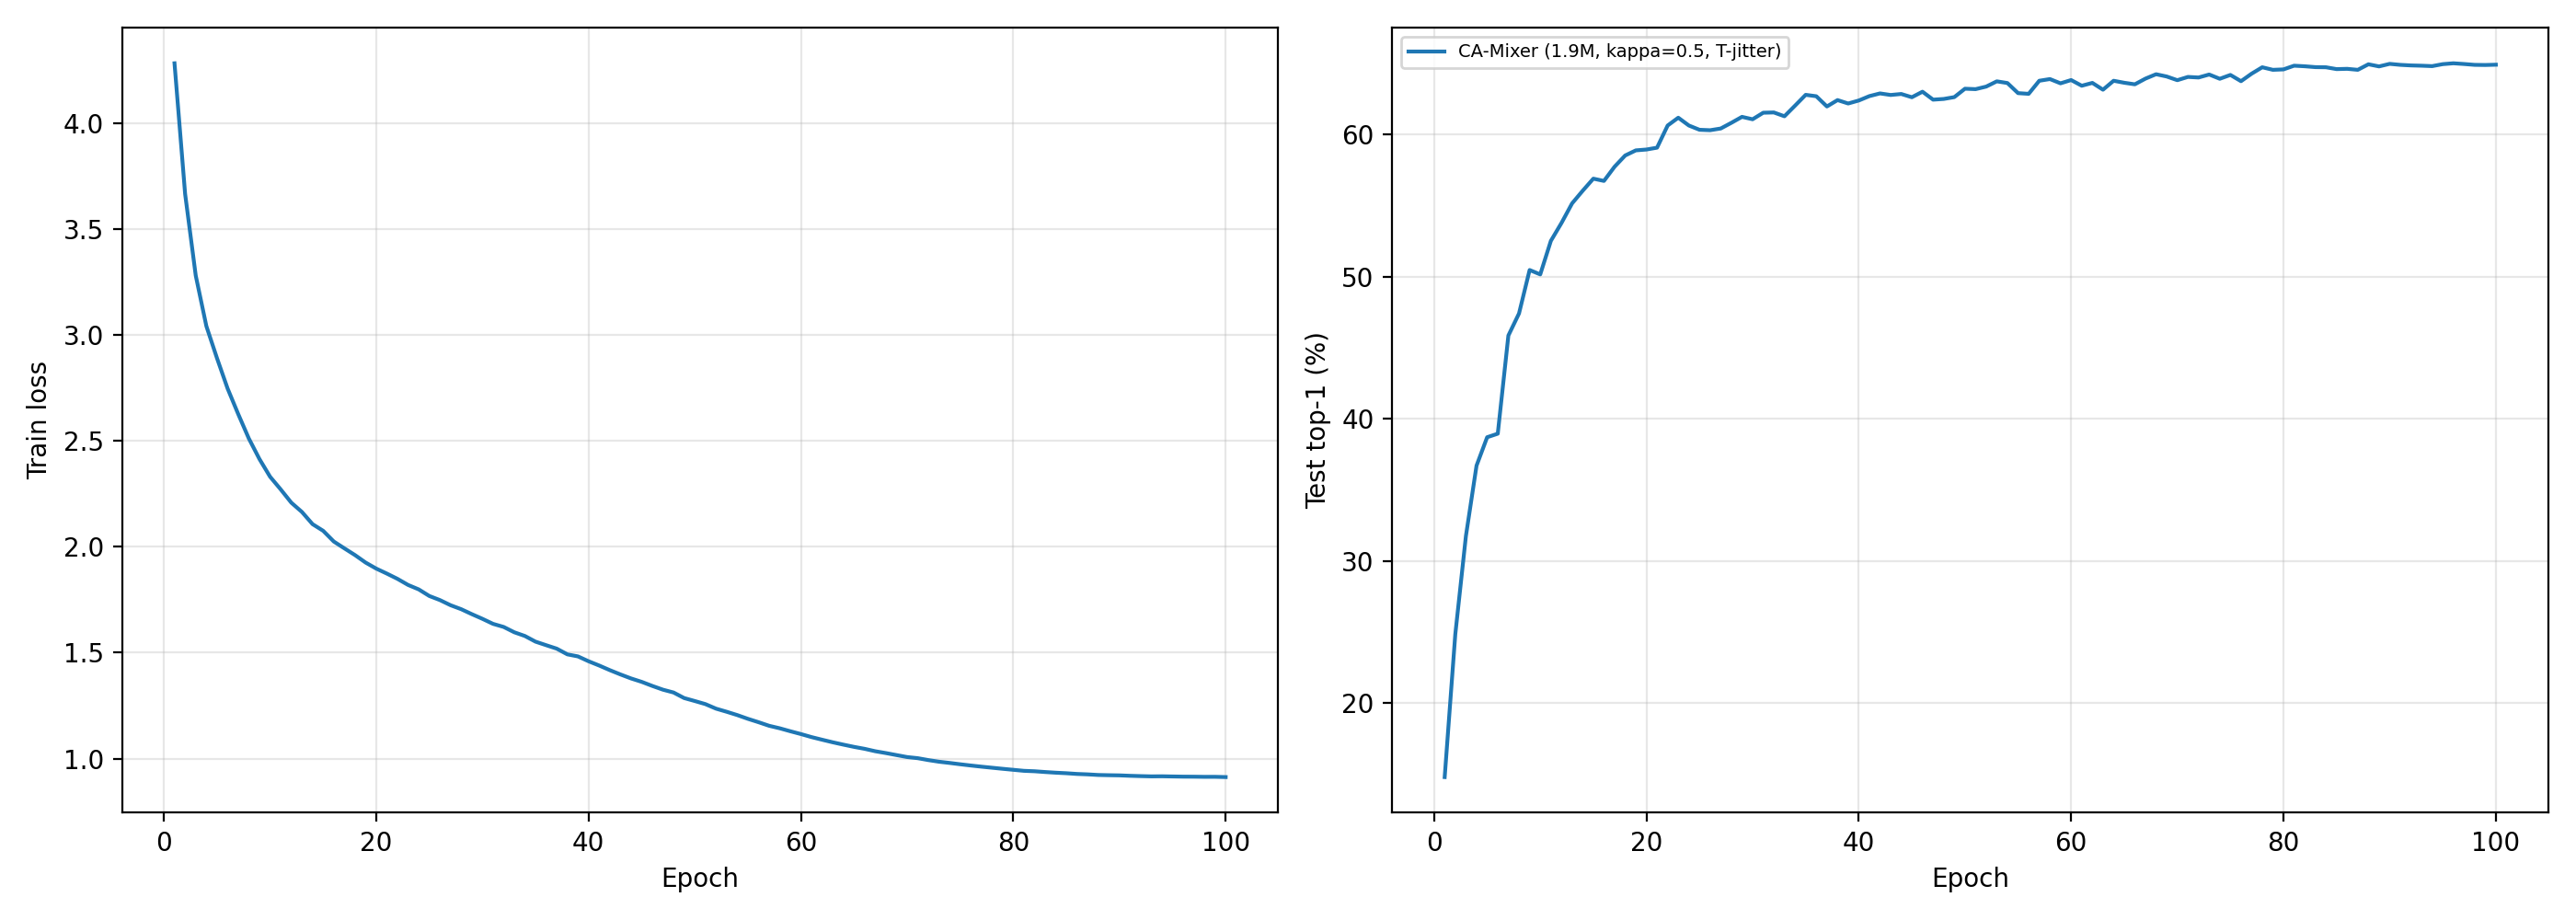
\includegraphics[width=0.98\textwidth]{figures/ca_100ep_training_curves.png}
\caption{Training loss (left) and test Top-1 validation accuracy (right) trajectories of CA-Mixer (1.90M parameters, $\kappa=0.5$, $T$-jitter) across 100 epochs on CIFAR-100.}
\label{fig:ca_100ep_curves}
\end{figure}

\subsubsection{Extended 300-Epoch Trajectory in HybridFormer}
In HybridFormer, the inclusion of multi-head self-attention in Stages 2 and 3 necessitates a longer optimization schedule. While the model reaches 65\% accuracy around epoch 100, continued training enables the attention layers to refine long-range semantic dependencies, ultimately peaking at \textbf{75.70\%} validation accuracy at epoch 275 and achieving \textbf{75.27\%} on the held-out test set.

\subsection{Scaling to Tiny-ImageNet (\texorpdfstring{$64 \times 64$}{64x64}, 200 Classes)}
To evaluate whether the pyramid architecture scales to higher spatial dimensions and larger class counts, we benchmarked Pyramid-ResMLP on Tiny-ImageNet across two distinct structural and regularization configurations, summarized in Table~\ref{tab:tiny_imagenet_scaling}:
\begin{itemize}
    \item \textbf{Base Configuration ($C=[96, 192, 384]$, $B=[2, 4, 6]$):} Containing 9.37M deployable parameters, the base model achieved 57.85\% Top-1 validation accuracy. However, signs of overfitting emerged as training accuracy reached 69.08\% while validation loss began to plateau around 2.0546.
    \item \textbf{Scaled Configuration with DropPath ($C=[112, 224, 448]$, $B=[2, 4, 6]$):} Increasing channel capacity to 12.73M deployable parameters while introducing stochastic depth ($\text{DropPath} = 0.05$), higher weight decay ($\lambda = 0.10$), and random erasing ($p=0.25$) improved Top-1 accuracy to \textbf{62.93\%} (and Top-5 accuracy to \textbf{82.83\%}). The $+5.08\%$ improvement confirms that stochastic depth effectively regularizes multi-stage pyramid MLPs on higher-resolution inputs.
\end{itemize}

\begin{table}[htbp]
\centering
\small
\begin{tabularx}{\textwidth}{l >{\raggedright\arraybackslash}X r r r}
\toprule
\textbf{Model Configuration} & \textbf{Channels, Depths, and Regularization} & \textbf{Deploy Params} & \textbf{Top-1 Val} & \textbf{Top-5 Val} \\
\midrule
Pyramid-ResMLP (Base) & $C=[96, 192, 384]$, $B=[2, 4, 6]$, $\lambda=0.05$ & 9,370,760 & 57.85\% & 79.12\% \\
\textbf{Pyramid-ResMLP (DropPath)} & $C=[112, 224, 448]$, $B=[2, 4, 6]$, DropPath 0.05, Erase 0.25 & \textbf{12,728,104} & \textbf{62.93\%} & \textbf{82.83\%} \\
\bottomrule
\end{tabularx}
\vspace{0.4em}
\caption{High-resolution scaling benchmark of Pyramid-ResMLP on Tiny-ImageNet ($64 \times 64$, 200 classes) across 100 epochs.}
\label{tab:tiny_imagenet_scaling}
\end{table}

\subsection{Hypothesis Verification: Resolving Parameter Inefficiency}
Our empirical findings definitively answer the research question formulated at the end of Week 02:

\subsubsection{The Two-Step Ablation Proof}
By comparing vanilla ResMLP, Pyramid-ResMLP Pure, and Pyramid-ResMLP, we isolate the exact source of performance gains:
\begin{align}
\text{ResMLP Isotropic (62.40\%)} &\xrightarrow{\mathbf{+5.82\%}} \text{Pyramid-ResMLP Pure (68.22\%)} \nonumber \\
&\xrightarrow{\mathbf{+3.96\%}} \text{Pyramid-ResMLP (72.18\%)}.
\end{align}
\begin{enumerate}
    \item \textbf{Step 1 (Hierarchical Pyramid):} Transitioning from a single-scale column to a 3-stage pyramid improves Top-1 accuracy by \textbf{+5.82\%} while saving 265k parameters and reducing training time from 54.65 to 44.91 minutes. This confirms that multi-scale downsampling provides crucial spatial abstraction.
    \item \textbf{Step 2 (Structural Re-parameterization):} Adding parallel depthwise convolutions during training contributes an additional \textbf{+3.96\%}. Because these branches fuse into the linear layer upon deployment, this gain incurs \textbf{zero inference latency or parameter overhead}.
\end{enumerate}

\subsubsection{Shift-ResMLP vs. Pyramid-ResMLP Tradeoff}
Shift-ResMLP demonstrates that spatial communication can achieve \textbf{72.92\%} accuracy with strictly zero learnable spatial weights. However, because Shift-ResMLP remains an isotropic columnar model, it requires 14.26M parameters and 110.21 minutes of training to achieve this score. In contrast, Pyramid-ResMLP reaches 72.18\% with only \textbf{1.79M deployable parameters} (an 8-fold reduction in parameter size) and trains in less than half the time (44.53 minutes), establishing hierarchical feature downsampling as the superior architectural paradigm.
